\documentclass[10pt, conference]{IEEEtran}
\usepackage[english]{babel}
\usepackage[usenames]{color}
\usepackage{colortbl}
\usepackage{comment}
\usepackage{graphicx}
\graphicspath{ {./images/} }
\usepackage{epsfig}
\usepackage{array, colortbl}
\usepackage{listings}
\usepackage{epstopdf}
\usepackage{multirow}
\usepackage{rotating}
%\usepackage{subfigure}
\usepackage{subfig}
\usepackage{float}
\usepackage[obeyspaces,hyphens,spaces]{url}
\usepackage{balance}
\usepackage{fancybox}
\usepackage{scalefnt}
\usepackage[normalem]{ulem}
%\pagestyle{plain}
\pagenumbering{arabic}
\pagestyle{empty}
\clubpenalty = 10000
\widowpenalty = 10000
\displaywidowpenalty = 10000
\usepackage{cleveref}
\usepackage{csquotes}

\makeatletter
\renewcommand{\paragraph}[1]{\noindent\textsf{#1}.}

\title{What automated Devops tools can help better understand clients needs 
  throughout the Devops cycle?}
\author{Billy Bouchard, Nicolas Legros    \\
    \emph{billy.bouchard@polymtl.ca, nicolas.legros@polymtl.ca}}

\begin{document}
\maketitle

\begin{abstract}
Lorem ipsum dolor sit amet, consectetur adipiscing elit. Nam nibh nisi, ultricies a placerat id, pharetra quis arcu. Donec ut rhoncus odio, in luctus turpis. Praesent in tellus in tellus volutpat sagittis non in felis. Praesent commodo, nisl ac ornare porta, quam libero consectetur mi, sed facilisis elit enim non ipsum. Ut consequat eros id ultricies iaculis. Ut pellentesque rhoncus neque. Integer vestibulum ac diam vitae faucibus. Sed sit amet viverra enim. Suspendisse eu nulla vel turpis auctor posuere sit amet non metus.
\end{abstract}

\section{Problem Statement \& Link with Course}
\label{sec:statement}

As all sofware exist to serve a client, wether internal or external, it is critical that they are developped with that in mind.
However, once the software goes live, updates are always necessary to patch some small bugs and add interesting feature.
It can be hard to see what features would be the best or which ones have been added with little to no succes or usage.
Moreover, developers sometimes work on features for a long time before validating their relevance to their clients. 
there is also the fact that testing new features or confirming feature success by getting customers' feedback can require the creation of focus groups, surveys or other more complex systems.
Using devops to create, receive and analyse customer feedbacks in a timely fashion would therefore help better the success of any software.
Indeed, automation of some customer feedbacks technic and their metrics analysis couls give the edge that a company need in order to successfully.

\section{Research Questions \& Motivation}
\label{sec:research-idea}

Knowing that the focus of this research will be on the automation of different technique, it should come to no suprise that the first part of the research will be to find the that can actually be automated.
\begin{displayquote}
  RQ1. \emph{What feedback techniques can be automatically operated throughout the Devops cycle?}.
\end{displayquote} 
Once there is a sufficient amount of information found on technics, we will focus on the different metrics leading to RQ2.
\begin{displayquote}
  RQ2. \emph{What feedback metrics can be automatically gathered and processed through logs or other Devops tools and metrics?}.
\end{displayquote} 
Once the compendium of both the techniques and the metrics can be found, we will be able to focsu a bit more on their individual usage to see how they are currently used which lead to RQ3.
\begin{displayquote}
  RQ2. \emph{How often are these techniques and metrics implemented in Devops projects?}.
\end{displayquote} 

All these considered, we should be able to better explain what techniques seems to be both easier to implemented and yield the best results. 


\section{Data Set \& Analyses}
\label{sec:backgr-relat-work}

Phasellus laoreet ipsum non nunc sodales molestie. Aliquam rutrum urna ante, at dictum odio dictum in. Quisque sit amet lorem non mi adipiscing aliquam. Suspendisse potenti. Aenean congue a risus vel posuere. Vestibulum tempor commodo ipsum vitae congue. Nunc vestibulum volutpat sapien quis tincidunt. Vestibulum vitae ullamcorper eros. Integer luctus quam risus~\cite{humble10}. Suspendisse scelerisque nulla nulla, sed ullamcorper enim faucibus sed. Curabitur bibendum ipsum quis justo tincidunt, et pulvinar enim ullamcorper. Pellentesque et tempor turpis. Pellentesque vel nisi metus. Proin laoreet vehicula vestibulum. Vivamus iaculis urna velit, et pharetra risus scelerisque quis~\cite{baysal11}.

\section{Two Related Papers}
\label{sec:two-related-papers}

This research shall be interisting due to the fact that not a lot of scholar articles exists on the subject.
However a ton of corporate article do exists and explain some core contexts 
One of the most interesting paper for this research as been written by google and can be found at this address: $https://cloud.google.com/architecture/devops/devops-process-customer-feedback$.
this article explain common metrics that google uses throughout their devops cycle. 
It goes into the details to explain the importance of both speed and regularity when it comes to customer feedbacks.
Their 5 most importants metrcis which are Acquisition(The percentage of users that come to your site who create an account),
Activation (The percentage of acquired users that activate their account and use the service),
Retention (The percentage of activated users that return to the service),
Referral (The percentage of retained users who refer other users to the service),
Revenue (The percentage of referring users who actually pay money for the service).
This corporate article is one of the numerous that explain well how to scales the devops pratices to include customers into the process.

Another really interesting articles that comes from the scholar sides is one from A. Fabijan et al. that is named \'Customer feedback and data collection techniques in software R\&D: A literature review\'. 
This article goes in depth to find all the different techniques and metrics that they could find to qualify and quantitfy customer feedback. 
It gives an incredibly thourough start point to see what technic and metrics this study should analyses and rank.
They explain both the stages at which they must be built, but also what limitation each technic faces.
Therefore, it will be easy to focus on the technic that can be included inside the devops cycle as both automated or semi-automated approach.

\section{Time Planning of Project}
\label{sec:schedule}

The timeline sees us providing the whole written report by the 22 dec and has us do a poster by the 28 of November. 
It was decided to do a backward analysis to get the most amount of time for each part of the project.
We shall keep the last month to simply right down the report once the poster is completed.
Therefore, a weekend would be kept to finish and complete the poster having the research completed by the 25 of November.
As the metrics evaluation should be done once the technique evaluation would be completed, the metrics evaluation would start one week before on the 19 of november.
It would then do great to allocate a total of 2 weeks to grab all the information on the metrics meanting the start of the metrics analysis part of our research on the 5 of November.
This means that the technique analysis part of our project would be completed by then.
It gives a total of 4 weeks to complete the technique analysis. the completed timline can be seen at figure \ref{fig:timline}.

\begin{figure}[h]
  \caption{projected timeline for the project}
  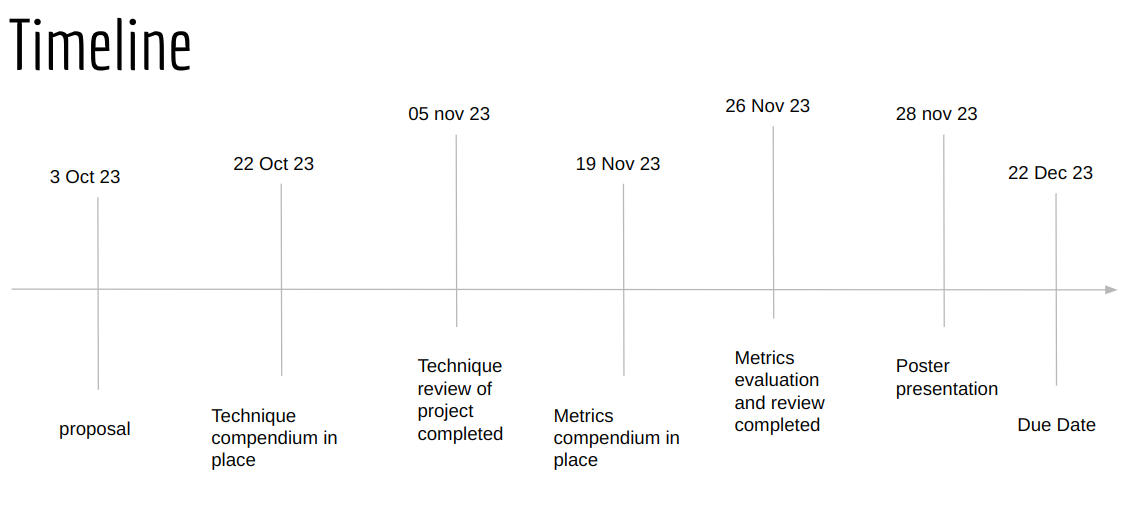
\includegraphics[width=0.5\textwidth]{timeline}
  \label{fig:timline}
\end{figure}

\balance
\bibliographystyle{IEEEtran}
\bibliography{proposal.bib}
\end{document}
